\documentclass[a4paper, 12pt]{article}
\usepackage[utf8]{inputenc}
\usepackage[english, ukrainian]{babel}

\usepackage{amsmath, amssymb}
\usepackage{multicol}
\usepackage{graphicx}
\usepackage{float}

\allowdisplaybreaks
\setlength\parindent{0pt}
\numberwithin{equation}{subsection}

\usepackage{hyperref}
\hypersetup{unicode=true,colorlinks=true,linktoc=all,linkcolor=red}

\numberwithin{equation}{subsection}

\renewcommand{\bf}[1]{\textbf{#1}}
\renewcommand{\it}[1]{\textit{#1}}
\newcommand{\bb}[1]{\mathbb{#1}}
\renewcommand{\cal}[1]{\mathcal{#1}}

\renewcommand{\epsilon}{\varepsilon}
\renewcommand{\phi}{\varphi}

\DeclareMathOperator{\diam}{diam}
\DeclareMathOperator{\rang}{rang}
\DeclareMathOperator{\const}{const}

\newenvironment{system}{%
  \begin{equation}%
    \left\{%
      \begin{aligned}%
}{%
      \end{aligned}%
    \right.%
  \end{equation}%
}
\newenvironment{system*}{%
  \begin{equation*}%
    \left\{%
      \begin{aligned}%
}{%
      \end{aligned}%
    \right.%
  \end{equation*}%
}

\makeatletter
\newcommand*{\relrelbarsep}{.386ex}
\newcommand*{\relrelbar}{%
  \mathrel{%
    \mathpalette\@relrelbar\relrelbarsep%
  }%
}
\newcommand*{\@relrelbar}[2]{%
  \raise#2\hbox to 0pt{$\m@th#1\relbar$\hss}%
  \lower#2\hbox{$\m@th#1\relbar$}%
}
\providecommand*{\rightrightarrowsfill@}{%
  \arrowfill@\relrelbar\relrelbar\rightrightarrows%
}
\providecommand*{\leftleftarrowsfill@}{%
  \arrowfill@\leftleftarrows\relrelbar\relrelbar%
}
\providecommand*{\xrightrightarrows}[2][]{%
  \ext@arrow 0359\rightrightarrowsfill@{#1}{#2}%
}
\providecommand*{\xleftleftarrows}[2][]{%
  \ext@arrow 3095\leftleftarrowsfill@{#1}{#2}%
}
\makeatother

\newcommand{\NN}{\mathbb{N}}
\newcommand{\ZZ}{\mathbb{Z}}
\newcommand{\QQ}{\mathbb{Q}}
\newcommand{\RR}{\mathbb{R}}
\newcommand{\CC}{\mathbb{C}}

\newcommand{\Max}{\displaystyle\max\limits}
\newcommand{\Sup}{\displaystyle\sup\limits}
\newcommand{\Sum}{\displaystyle\sum\limits}
\newcommand{\Int}{\displaystyle\int\limits}
\newcommand{\Iint}{\displaystyle\iint\limits}
\newcommand{\Lim}{\displaystyle\lim\limits}

\newcommand*\diff{\mathop{}\!\mathrm{d}}

\newcommand*\rfrac[2]{{}^{#1}\!/_{\!#2}}


\title{{\Huge МАТЕМАТИЧНА ФІЗИКА}}
\author{Скибицький Нікіта}
\date{\today}

\usepackage{amsthm}
\usepackage[dvipsnames]{xcolor}
\usepackage{thmtools}
\usepackage[framemethod=TikZ]{mdframed}

\theoremstyle{definition}
\mdfdefinestyle{mdbluebox}{%
	roundcorner = 10pt,
	linewidth=1pt,
	skipabove=12pt,
	innerbottommargin=9pt,
	skipbelow=2pt,
	nobreak=true,
	linecolor=blue,
	backgroundcolor=TealBlue!5,
}
\declaretheoremstyle[
	headfont=\sffamily\bfseries\color{MidnightBlue},
	mdframed={style=mdbluebox},
	headpunct={\\[3pt]},
	postheadspace={0pt}
]{thmbluebox}

\mdfdefinestyle{mdredbox}{%
	linewidth=0.5pt,
	skipabove=12pt,
	frametitleaboveskip=5pt,
	frametitlebelowskip=0pt,
	skipbelow=2pt,
	frametitlefont=\bfseries,
	innertopmargin=4pt,
	innerbottommargin=8pt,
	nobreak=true,
	linecolor=RawSienna,
	backgroundcolor=Salmon!5,
}
\declaretheoremstyle[
	headfont=\bfseries\color{RawSienna},
	mdframed={style=mdredbox},
	headpunct={\\[3pt]},
	postheadspace={0pt},
]{thmredbox}

\declaretheorem[style=thmbluebox,name=Теорема,numberwithin=subsubsection]{theorem}
\declaretheorem[style=thmbluebox,name=Лема,numberwithin=subsubsection]{lemma}
\declaretheorem[style=thmbluebox,name=Твердження,numberwithin=subsubsection]{proposition}
\declaretheorem[style=thmbluebox,name=Принцип,numberwithin=subsubsection]{th_principle}
\declaretheorem[style=thmbluebox,name=Закон,numberwithin=subsubsection]{law}
\declaretheorem[style=thmbluebox,name=Закон,numbered=no]{law*}
\declaretheorem[style=thmbluebox,name=Формула,numberwithin=subsubsection]{th_formula}
\declaretheorem[style=thmbluebox,name=Рівняння,numberwithin=subsubsection]{th_equation}
\declaretheorem[style=thmbluebox,name=Умова,numberwithin=subsubsection]{th_condition}
\declaretheorem[style=thmbluebox,name=Наслідок,numberwithin=subsubsection]{corollary}

\declaretheorem[style=thmredbox,name=Приклад,numberwithin=subsubsection]{example}
\declaretheorem[style=thmredbox,name=Приклади,sibling=example]{examples}

\declaretheorem[style=thmredbox,name=Властивість,numberwithin=subsubsection]{property}
\declaretheorem[style=thmredbox,name=Властивості,sibling=property]{properties}

\mdfdefinestyle{mdgreenbox}{%
	skipabove=8pt,
	linewidth=2pt,
	rightline=false,
	leftline=true,
	topline=false,
	bottomline=false,
	linecolor=ForestGreen,
	backgroundcolor=ForestGreen!5,
}
\declaretheoremstyle[
	headfont=\bfseries\sffamily\color{ForestGreen!70!black},
	bodyfont=\normalfont,
	spaceabove=2pt,
	spacebelow=1pt,
	mdframed={style=mdgreenbox},
	headpunct={ --- },
]{thmgreenbox}

\mdfdefinestyle{mdblackbox}{%
	skipabove=8pt,
	linewidth=3pt,
	rightline=false,
	leftline=true,
	topline=false,
	bottomline=false,
	linecolor=black,
	backgroundcolor=RedViolet!5!gray!5,
}
\declaretheoremstyle[
	headfont=\bfseries,
	bodyfont=\normalfont\small,
	spaceabove=0pt,
	spacebelow=0pt,
	mdframed={style=mdblackbox}
]{thmblackbox}

\declaretheorem[name=Вправа,numberwithin=subsubsection,style=thmblackbox]{exercise}
\declaretheorem[name=Зауваження,numberwithin=subsubsection,style=thmgreenbox]{remark}
\declaretheorem[name=Визначення,numberwithin=subsubsection,style=thmblackbox]{definition}

\newtheorem{problem}{Задача}[subsection]
\newtheorem{sproblem}[problem]{Задача}
\newtheorem{dproblem}[problem]{Задача}
\renewcommand{\thesproblem}{\theproblem$^{\star}$}
\renewcommand{\thedproblem}{\theproblem$^{\dagger}$}
\newcommand{\listhack}{$\empty$\vspace{-2em}} 

\theoremstyle{remark}
\newtheorem*{solution}{Розв'язок}


\begin{document}

\tableofcontents

\setcounter{section}{3}
\setcounter{subsection}{2}
\setcounter{subsubsection}{5}
\setcounter{theorem}{22}
\setcounter{equation}{56}

Порівнюючи формули переходу до нових координат для обох тензорів, бачимо їх ідентичність, тобто перетворення тензора напружень та тензору деформацій відбувається за однаковими формулами. Таким чином існує система координат $h_1$, $h_2$, $h_3$, для якої тензор деформації має діагональний вигляд: 
\begin{equation}
	\begin{pmatrix}
		\epsilon_1 & 0 & 0 \\
		0 & \epsilon_2 & 0 \\
		0 & 0 & \epsilon_3.
	\end{pmatrix}
\end{equation}

\begin{definition}[головних компонент тензора деформацій]
 	$\epsilon_1$, $\epsilon_2$, $\epsilon_3$ називаються \it{головними компонентами} тензора деформацій.
\end{definition} 

\begin{definition}[головних вісей тензора деформацій]
	$h_1$, $h_2$, $h_3$ називаються \it{головними вісями} тензора деформацій.
\end{definition}

З формули переходу можна отримати зв'язок між компонентами тензору деформацій у прямокутній системі координат $x$, $y$, $z$ та головними компонентами тензору деформацій:
\begin{align}
	\gamma_{a b} &= \Sum_{i = 1}^3 2 \epsilon_i \cos (h_i, a) \cos (h_i, b), \\
	\epsilon_a &= \Sum_{i = 1}^3 \epsilon_i \cos^2(h_i, a),
\end{align}
де $a, b \in \{x, y, z\}$. \medskip

Без доведення приймемо до уваги 

\begin{proposition}
	Для ізотропних тіл (тіл властивості яких в усіх напрямках однакові) головні вісі тензора деформації та тензора напружень співпадають:
	\begin{align}
		\tau_{a b} &= \Sum_{i = 1}^3 2 \epsilon_i \cos (h_i, a) \cos (h_i, b), \\
		\sigma_a &= \Sum_{i = 1}^3 \epsilon_i \cos^2(h_i, a),
	\end{align}
	де $a, b \in \{x, y, z\}$.
\end{proposition}

\subsubsection{Закон Гука. Зв'язок між тензором деформації та тензором напружень}

Розглянемо пружній паралелепіпед до нижньої грані якого прикладене напруження $\sigma_1$ у напряму першої головної координатної вісі $h_1$:
\begin{figure}[H]
	\centering
	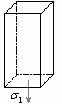
\includegraphics[]{img/9-1.png}
\end{figure}

Згідно до спрощеного трактування закону Гука  
\begin{equation}
	\epsilon_1 = \frac{\sigma_1}{E},
\end{equation}
де $E$ --- \it{модуль Юнга}. \medskip

При подовжені паралелепіпеду у напрямку першої координатної вісі $h_1$, відбувається стиснення паралелепіпеду у напрямах двох інших головних вісей і це стиснення пропорційне прикладеному напруженню $\sigma_1$. \medskip

Прикладаючи напруження в напряму двох інших головних координатних вісей $\sigma_2$ та $\sigma_3$, відповідно будемо мати стиснення в напряму $h_1$. Це від'ємне подовження (стиснення) в напрямку першої координатної вісі, за рахунок напруження $\sigma_2$ дорівнює $\sigma_2 / m E$, а за рахунок напруження $\sigma_3$ дорівнює $\sigma_3 / m E$. \medskip

Отже, маємо 
\begin{law}[Гука, загальний]
	Повна величина подовження в напрямку першої головної координатної вісі дорівнює
	\begin{equation}
		\epsilon_1 = \frac{1}{E} \left( \sigma_1 - \frac{\sigma_2 + \sigma_3}{m} \right) = \frac{m + 1}{E m} \left( \sigma_1 - \frac{\sigma_1 + \sigma_2 + \sigma_3}{m + 1} \right)
	\end{equation}
\end{law}

Позначимо $S = \sigma_1 + \sigma_2 + \sigma_3$ і запишемо 
\begin{law}[Гука]
	Зв'язок між головними компонентами тензора напружень та тензора деформації:
	\begin{equation}
		\epsilon_i = \frac{m + 1}{E m} \left( \sigma_i - \frac{S}{m + 1} \right),
	\end{equation}
	для $i = 1, 2, 3$.
\end{law}

Використовуючи формули переходу до нової системи координат отримаємо:
\begin{equation}
	\begin{aligned}
		\epsilon_x &= \Sum_{i = 1}^3 \frac{m + 1}{E m} \left( \sigma_i - \frac{S}{m + 1} \right) \cos^2( h_i, x ) = \\
		&= \frac{m + 1}{E m} \left(\Sum_{i = 1}^3 \sigma_i \cos^2(h_i, x) - \frac{S}{m + 1} \Sum_{i = 1}^3 \cos^2(h_i, x)\right) =\\
		&= \frac{m + 1}{E m} \left( \sigma_x - \frac{S}{m + 1} \right).
	\end{aligned}
\end{equation}

Неважко перевірити, що 
\begin{equation}
	S = \sigma_1 + \sigma_2 + \sigma_3 = \sigma_x + \sigma_y + \sigma_z,
\end{equation}
тобто $S$ --- інваріант для різних прямокутних систем координат. \medskip

Для поза діагональних елементів, зв'язок між компонентами тензора деформацій і тензора напружень має вигляд:
\begin{equation}
	\gamma_{x y} = \frac{2 (m + 1)}{E m} \sum_{i = 1}^3 \left( \sigma_i - \frac{S}{m + 1} \right) \cos (h_i, x) \cos (h_i, y) = \frac{2 (m + 1)}{E m} \cdot \tau_{x y}.
\end{equation}
 
Позначимо $G = E m / 2 (m + 1)$ та запишемо 
\begin{law}[Гука для будь-якої прямокутної системи координат]
	Залежність між тензором деформацій та тензором напружень у довільній прямокутній системі координат:
	\begin{align}
		\epsilon_a &= \frac{1}{2 G} \left(\sigma_a - \frac{S}{m + 1}\right), \\
		\gamma_{\alpha \beta} &= \frac{\tau_{\alpha \beta}}{G},
	\end{align}
	де $\alpha, \beta \in \{x, y, z\}$.
\end{law}

Запишемо обернену залежність тензора напружень від тензора деформації, нехай
\begin{equation}
	\theta = \epsilon_x + \epsilon_y + \epsilon_z = \frac{1}{2G} \left( S - \frac{3 S}{m + 1} \right) = \frac{1}{2 G} \left( \frac{(m - 2) S}{m +1} \right),
\end{equation}
тоді
\begin{equation}
	S = \frac{2 \theta (m + 1) G}{m - 2}.
\end{equation}

Таким чином можна записати
\begin{equation}
	\sigma_x = 2 G \epsilon_x + \frac{S}{m + 1} = 2 G \epsilon_x + \frac{2 G \theta}{m - 2} = 2 G \left( \epsilon_x + \frac{\theta}{m - 2} \right).
\end{equation}

В результаті маємо 
\begin{law}[Гука, еквівалентна форма]
	Для довільної прямокутної системи координат:
	\begin{align}
		\sigma_\alpha &= 2 G \left( \epsilon_\alpha + \frac{\theta}{m - 2} \right), \\
		\tau_{\alpha \beta} &= G \gamma_{\alpha \beta},
	\end{align}
	де $\alpha, \beta \in \{x, y, z\}$.
\end{law}

Запишемо замкнену систему диференціальних рівнянь, яка складається з останніх рівнянь, закону рівноваги елементу об'єму
\begin{system}
	\frac{\partial \sigma_x}{\partial x} + \frac{\partial \tau_{x y}}{\partial y} + \frac{\partial \tau_{x z}}{\partial z} + X &= 0, \\
	\frac{\partial \tau_{y x}}{\partial x} + \frac{\partial \sigma_y}{\partial y} + \frac{\partial \tau_{y z}}{\partial z} + Y &= 0, \\
	\frac{\partial \tau_{z x}}{\partial x} + \frac{\partial \tau_{z y}}{\partial y} + \frac{\partial \sigma_z}{\partial z} + Z &= 0.
\end{system}
і виразів які зв'язують компоненти тензору деформацій та вектор переміщень:
\begin{system}
	\gamma_{x y} &= \frac{\partial V}{\partial x} + \frac{\partial U}{\partial y} = \gamma_{y x}, \\
	\gamma_{x z} &= \frac{\partial W}{\partial x} + \frac{\partial U}{\partial z} = \gamma_{z x}, \\
	\gamma_{y z} &= \frac{\partial W}{\partial y} + \frac{\partial V}{\partial z} = \gamma_{z y}, \\
	\epsilon_x &= \frac{\partial U}{\partial x}, \\
	\epsilon_y &= \frac{\partial V}{\partial y}, \\
	\epsilon_z &= \frac{\partial W}{\partial z}.
\end{system}

Всі ці співвідношення складають систему п'ятнадцяти лінійних диференціальних рівнянь з п'ятнадцятьма невідомими функціями. \medskip

Найчастіше цю систему перетворюють до вигляду трьох рівнянь з трьома невідомими відносно вектора переміщень. Для здійснення перетворень з першої і третьої груп рівнянь виключимо тензор деформацій, та підставимо отриманий вираз для напружень через переміщення у другу групу рівнянь, отримаємо статичну систему теорії пружності.

\begin{th_equation}[статичні рівняння теорії пружності]
	Напружено-деформований стан тіла, при умові що воно знаходиться у стані спокою або рівномірного і прямолінійного руху, описується системою
	\begin{equation}
		G \left( \Delta \vec U + \frac{m}{m - 2} \nabla \left(\nabla \cdot \vec U\right) \right) + \vec X = 0,
	\end{equation}
	де $(x, y, z) \in \Omega$.
\end{th_equation}

У випадку, коли одні частини тіла рухаються відносно інших, замість статичних рівнянь теорії пружності мають місце 
\begin{th_equation}[динамічні рівняння теорії пружності]
	Напружено-деформований стан тіла, коли одні частини тіла рухаються відносно інших, описується системою
	\begin{equation}
		G \left( \Delta \vec U + \frac{m}{m - 2} \nabla \left(\nabla \cdot \vec U\right) \right) + \vec X = \rho \cdot \frac{\partial^2 \vec U}{\partial t^2},
	\end{equation}
	де $(x, y, z) \in \Omega$ і $ t > 0$.
\end{th_equation}

\begin{remark}
	Остання система рівнянь може бути отримана, якщо використати більш загальний вигляд закону рівноваги елементу об'єму в якому рівнодіюча поверхневих та об'ємних сил дорівнюють силі інерції (другий закон Ньютона):
	\begin{system}
		\frac{\partial \sigma_x}{\partial x} + \frac{\partial \tau_{x y}}{\partial y} + \frac{\partial \tau_{x z}}{\partial z} + X &= \rho \cdot \frac{\partial^2 U}{\partial t^2}, \\
		\frac{\partial \tau_{y x}}{\partial x} + \frac{\partial \sigma_y}{\partial y} + \frac{\partial \tau_{y z}}{\partial z} + Y &= \rho \cdot \frac{\partial^2 V}{\partial t^2}, \\
		\frac{\partial \tau_{z x}}{\partial x} + \frac{\partial \tau_{z y}}{\partial y} + \frac{\partial \sigma_z}{\partial z} + Z &= \rho \cdot \frac{\partial^2 W}{\partial t^2}.
	\end{system}
	де права частина формули представляє силу інерції.
\end{remark}

\subsubsection{Початкові та граничні умови для рівнянь теорії пружності}

Для нестаціонарної системи теорії пружності в початковий момент часу необхідно задавати вектор переміщень
\begin{equation}
	\vec U(x, y, z, 0) = \vec U_0(x, y, z)
\end{equation}
та вектор початкових швидкостей
\begin{equation}
	\frac{\partial \vec U(x, y, z, 0)}{\partial t} = \vec U_1(x, y, z).
\end{equation}

Перейдемо тепер до крайових (граничних) умов:
\begin{itemize}
	\item Якщо на границі області $(x, y, z) \in S = \partial \Omega$ відомий вектор зміщень, то задають граничні умови Діріхле.

	\begin{definition}[умов Діріхле]
		\it{Умовами Діріхле} називають співвідношення
		\begin{equation}
			\left. \vec U(x, y, z, t) \right|_{(x, y, z) \in S} = \vec W(x, y, z, t).
		\end{equation}
	\end{definition}

	\item Якщо на поверхні тіла відомий (заданий) вектор поверхневих сил, то в точках границі згідно закону рівноваги елементу поверхні задають умови для напрямку $x$:
	\begin{equation}
		\left. \Sum_{a \in \{x, y, z\}} \tau_{x a}\cos(\vec{\bf{n}}, a) \right|_{(x, y, z) \in S} = F_x(x, y, z, t).
	\end{equation}

	Аналогічно для напрямків $y$, $z$. Тобто маємо умови Неймана.

	\begin{definition}[умов Неймана]
		\it{Умовами Неймана} називають співвідношення
		\begin{equation}
			\left. \Sum_{a \in \{x, y, z\}} \tau_{b a} \cos(\vec{\bf{n}}, a) \right|_{(x, y, z) \in S} = F_b(x, y, z, t),
		\end{equation}
		 де $b \in \{x, y, z\}$.
	\end{definition}

	\item Якщо точки границі закріплені пружно, наприклад за допомогою пружини, то у цьому випадку на границю діє поверхнева сила пропорційна зміщенню точок тіла і направлена в бік протилежний зміщенню. Таким чином задаються граничні умови Ньютона.

	\begin{definition}[умов Ньютона]
		\it{Умовами Ньютона} називають співвідношення
		\begin{equation}
			\left. \Sum_{a \in \{x, y, z\}} \tau_{b a} \cos(\vec{\bf{n}}, a) \right|_{(x, y, z) \in S} = - K_b \cdot \left. U_b(x, y, z, t) \right|_{(x, y, z) \in S},
		\end{equation}
		де $b \in \{x, y, z\}$.
	\end{definition}

	\begin{remark}
		Тут $K_b$ --- коефіцієнт пропорційності (пружного закріплення).
	\end{remark}

	\item Якщо на тіло закріплено пружно одночасно дії зовнішня сила, то маємо неоднорідну граничну умову третього роду, яка запишеться у вигляді:
	\begin{multline}
		\left. \Sum_{a \in \{x, y, z\}} \tau_{b a} \cos(\vec{\bf{n}}, a) \right|_{(x, y, z) \in S} = \\
		= - K_b \cdot \left. \left( U_b(x, y, z, t) + F_b(x, y, z, t) \right) \right|_{(x, y, z) \in S},
	\end{multline}
	де $b \in \{\xi, y, z\}$.
\end{itemize}

\subsubsection{Спрощення системи рівнянь теорії пружності}

Відомо, що за теоремою Гельмгольца, векторне поле $\vec U$ завжди можна представити у вигляді суми потенціального та соліноїдального векторних полів. \medskip

Тобто існують така скалярна функція $\phi$ та векторна функція $\vec \Phi$, які називають скалярним та векторним потенціалами відповідно що
\begin{equation}
	\vec U = \nabla \phi + \nabla \times \vec \Phi.
\end{equation}

Для вектору масових сил $\vec X$ теж застосуємо представлення у вигляді потенціальної та соліноїдальної складових:
\begin{equation}
	\vec X = \nabla f + \nabla \times \vec F.
\end{equation}

Підставимо ці представлення у динамічні рівняння, отримаємо:
\begin{multline}
	\nabla \left( \left( \frac{2 G (m - 1)}{(m - 2)} \cdot \Delta \phi + f - \rho \cdot \frac{\partial^2 \phi}{\partial t^2} \right) \right) + \\
	+ \nabla \times \left( G \Delta \vec \Phi + \Vec F - \rho \cdot \frac{\partial^2 \vec \Phi}{\partial t^2} \right) = 0.
\end{multline}

В результаті маємо рівняння скалярне та векторне хвильове рівняння:
\begin{th_equation}[скалярне хвильове]
	Виконується співвідношення:
	\begin{equation}
		\rho \cdot \frac{\partial^2 \phi}{\partial t^2} = \left( \frac{2 G (m - 1)}{(m - 2)} \right) \Delta \phi + f.
	\end{equation}
\end{th_equation}

\begin{th_equation}[векторне хвильове]
	Виконується співвідношення:
	\begin{equation}
		\rho \cdot \frac{\partial^2 \vec \Phi}{\partial t^2} = G \Delta  \vec \Phi + \vec F.
	\end{equation}
\end{th_equation}

\subsubsection{Математична модель поздовжніх коливань стрижня}

Нехай маємо пружній стрижень, який витягнутий вздовж вісі $Ox$ і має довжину $L$. Відносно стрижня будемо припускати, що переміщення, деформації та напруження, які можуть виникати в стрижні направлені лише вздовж вісі $Ox$ і не залежать від інших просторових координат. \medskip

Зрозуміло, що в цьому випадку для компонентів тензора напружень можна записати: 
\begin{equation}
	\tau_{x y} = \tau_{y x} = \tau_{y z} = \sigma_y = \sigma_z = 0, \quad \sigma_x = \sigma_x(x, t).
\end{equation}

Будемо нехтувати також змінами поперечного перерізу при деформаціях вздовж вісі $Ox$. В цьому випадку закон Гука має вигляд: $\epsilon_x = \sigma_x / E$. \medskip

Спрощений вигляд закону рівноваги елементу об'єму з можна записати у вигляді
\begin{equation}
	\frac{\partial \sigma_x}{\partial x} + F_x(x, t) = \rho \cdot \frac{\partial^2 U}{\partial t^2}.
\end{equation}

Або враховуючи зв'язок тензора деформацій і вектору переміщень, будемо мати 
\begin{th_equation}[поздовжніх коливань стрижня]
	Виконується рівняння
	\begin{equation}
		\rho \cdot \frac{\partial^2 U}{\partial t^2} = E \cdot \frac{\partial^2 U}{\partial x^2} + F_x(x, t),
	\end{equation}
	де $0 < x < L$ і $t > 0$.
\end{th_equation}

В початковий момент часу необхідно задавати початкові змішення та початкові швидкості в напрямку вісі $Ox$:
\begin{align}
	U(x, 0) &= U_0(x), \\
	\frac{\partial U(x, 0)}{\partial t} &= U_1(x).
\end{align}

Розглянемо можливі граничні умови на правому кінці стрижня:
\begin{itemize}
	\item На правому кінці заданий закон його руху (зміщення):
	\begin{equation}
		U(L, t) = \phi_2(t).
	\end{equation}
	\item На правий кінець діє задана сила. Враховуючи, що $\vec{\bf{n}} = (1, 0, 0)$, можна записати $\sigma_x(L, t) = \psi_2(t)$, або, враховуючи спрощений закон Гука:
	\begin{equation}
		E \cdot \frac{\partial U(L, t)}{\partial x} = \psi_2(t).
	\end{equation}
	\item  Правий кінець закріплений пружно. Можемо записати $\sigma_x(L, t) + K_x \cdot U(L, t) = 0$, або враховуючи закон Гука:
	\begin{equation}
		E \cdot \frac{\partial U(L, t)}{\partial x} + K_x \cdot U(L, t) = 0.		
	\end{equation}
\end{itemize}

\subsubsection{Математична модель поперечних коливання струни}

Струною будемо називати абсолютно гнучку нитку, нескінченно малого поперечного перерізу, яка не протидії згинанню. \medskip

Нехай струна має довжину $L$ і в положенні рівноваги співпадає з відрізком вісі $Ox$, лівий кінець співпадає з початком координат. \medskip

Будемо вважати, що струна рівномірно натягнута з силою $T_0 = \const$, і може здійснювати коливання лише в одній площині. \medskip

Будемо розглядати лише малі коливання, тобто такі, коли відхилення точок струни від положення рівноваги є величинами першого порядку малості, при цьому величинами більш високого порядку малості будемо нехтувати. \medskip

Припущення про абсолютну гнучкість струни означає, що при відхиленні точок струни від положення рівноваги сила натягу весь час направлена по дотичній до миттєвого профілю струни. \medskip

Введемо позначення:
\begin{itemize}
	\item $\rho$ --- лінійна щільність точок струни ($\const$);
	\item $u(x, t)$ --- відхилення точок струни від положення рівноваги в точці $(x, t)$;
	\item $f(x, t)$ --- інтенсивність зовнішніх сил.
\end{itemize}

Запишемо рівняння руху для елементарної частини струни $(x, x + \Delta x)$ в проекції на вісь $u$. Підрахуємо наскільки змінилася довжина частини струни, між перерізами $x$ і $x + \Delta x$. Згідно до відомої формули математичного аналізу можемо записати, що довжина дуги обчислюється
\begin{equation}
	\diff s = \sqrt{(\diff x)^2 + (\diff u)^2} = \diff x \sqrt{1 + \left( \frac{\partial u}{\partial x} \right)^2} \approx \diff x.
\end{equation}

Таким чином зміною довжини дуги струни з точністю до членів другого порядку малості можна нехтувати. \medskip

Це в свою чергу означає, що за законом Гука сила натягу залишається постійною в кожному перерізі струни, тобто $T(x, t) = T_0$. \medskip

Виділимо сили, які діють на елементарну частину струни. \medskip

Проекція сили натягу в перерізі $x + \Delta x$ на вісь вздовж якої відбувається рух точок струни (вісь $u$) дорівнює $T_0 \sin \alpha (x + \Delta x, t) $, а в перерізі $x$ дорівнює $-T_0 \sin \alpha(x, t)$, де $\sin \alpha(x, t)$ --- синус кута між дотичною і додатнім напрямом вісі $x$. Для малих кутів $\sin \alpha \approx \tan \alpha = \partial u / \partial x$. \medskip

Таким чином рівнодіючу сил натягу можна записати у вигляді
\begin{equation}
	T_0(u_x(x + \Delta x, t) - u_x(x, t)).
\end{equation}

Зовнішня сила яка діє на виділений елемент струни дорівнює $f(\xi, t) \Delta x$. \medskip

Згідно до другого закону Ньютона рівнодіюча зовнішніх сил повинна дорівнювати силі інерції $F = ma$. \medskip

Сила інерції елементарного відрізка струни має вигляд:
\begin{equation}
	\rho \Delta x \frac{\partial^2 u(\xi, t)}{\partial t^2},	
\end{equation}
де $\xi$ --- якась середня точка, тобто $\xi \in (x, x + \Delta x)$. \medskip

Таким чином згідно до закону Ньютона можна записати рівняння руху:
\begin{equation}
	\rho \cdot \Delta x \cdot \frac{\partial^2 u(\xi, t)}{\partial t^2} = T_0(u_x(x + \Delta x, t) - u_x(x, t)) + f(\xi, t) \Delta x.
\end{equation}

Поділивши це рівняння на $\Delta x$ і спрямувавши його до нуля отримаємо 

\begin{th_equation}[коливання струни]
	Виконується рівняння
	\begin{equation}
		\rho \cdot \frac{\partial^2 u(x, t)}{\partial t^2} = T_0 \cdot \frac{\partial^2 u(x, t)}{\partial x^2} + f(x, t),
	\end{equation}
	де $0 < x < L$, і $t > 0$.
\end{th_equation}

Додаткові умови для рівняння коливання струни полягають в необхідності задавати початкове відхилення точок струни і початкові швидкості точок струни:
\begin{align}
	u(x, 0) &= u_0(x), \\
	\frac{\partial u(x, 0)}{\partial t} &= v_0(x),
\end{align}
для $0 < x < L$. \medskip

Окрім початкових умов необхідно задавати умови на кінцях струни. Найбільш поширеними умовами є:
\begin{itemize}
	\item Кінець струни рухаються за заданим законом;
	\item На кінець струни діє задана сила;
	\item Кінець струни закріплений пружно.
\end{itemize}

Запишемо відповідні граничні умови для випадку лівого кінця.
\begin{itemize}
	\item Якщо лівий кінець рухається за заданим законом, то 
	\begin{equation}
		u(0, t) = \phi_1(t).
	\end{equation}
	\item У випадку, коли на лівому кінці діє задана сила, то для отримання граничної умови  можна записати рівняння руху для елементарного відрізку $[0, \Delta x]$  яке матиме вигляд:
	\begin{equation}
		\rho \cdot \Delta x \cdot \frac{\partial^2 u(\xi, t)}{\partial t^2} = T_0 \cdot u_x(\Delta x, t) - \psi_1(t) + f(\xi, t),
	\end{equation}
	де $\xi$ --- якась середня точка, тобто $\xi \in (0, \Delta x)$. \medskip
 
	Спрямувавши $\Delta x \to 0$ отримаємо граничну умову 
	\begin{equation}
		u_x(0, t) = \frac{\psi_1(t)}{T_0}.
	\end{equation}

	\item Для випадку пружного закріплення замість заданої сили $\psi_1(t)$ необхідно розглядати силу реакції пружини, яка пропорційна зміщенню і діє в напрямку протилежному зміщенню. Таким чином рівняння руху буде мати вигляд:
	\begin{equation}
		\rho \cdot \Delta x \cdot \frac{\partial^2 u(\xi, t)}{\partial t^2} = T_0 \cdot u_x(\Delta x, t) + k \cdot u(0, t) + f(\xi, t),
	\end{equation}
	де $\xi$ --- якась середня точка, тобто $\xi \in (0, \Delta x)$. \medskip

	Після граничного переходу отримаємо 
	\begin{equation}
		u_x(0, t) + \frac{K}{T_0} \cdot u(0, t) = 0,	
	\end{equation}
	де $k$ --- коефіцієнт жорсткості пружини.
\end{itemize}

\end{document}